\documentclass[12pt]{article}
\usepackage{hyphenat}
\usepackage[top=2.6cm,bottom=2.6cm,left=2.8cm,right=2.8cm]{geometry}
\usepackage{amsmath,amssymb}
\usepackage{booktabs}
\usepackage[utf8]{inputenc}
\usepackage[T1]{fontenc}
\usepackage{lmodern}
\usepackage{microtype}
\usepackage{setspace}
\usepackage{graphicx}
\usepackage[hidelinks]{hyperref}
\usepackage{natbib}
\usepackage{caption}
\usepackage{threeparttable}
\usepackage{dcolumn}
\usepackage{footmisc}

\setstretch{1.25}

\title{\textbf{Do Voters Punish Gasoline Price Shocks?\\
Evidence from U.S.\ Midterm Elections, 1994--2022}}

\author{Alejandro Corch\'on Franco\\[4pt]
\small Faculty of Economics and Business\\
\small Universitat Pompeu Fabra\\[2pt]
\small \texttt{alejandro.corchon01@estudiant.upf.edu}}

\date{}

\begin{document}
\maketitle
\thispagestyle{empty}

% ── Abstract ──────────────────────────────────────────────────────────────────

\begin{abstract}
\noindent
This paper examines whether retail gasoline prices affect the electoral performance of the U.S. presidential party in midterm House elections. Using a state-by-election-year panel for 1994--2022, I identify the effect of gasoline prices through their interaction with predetermined state-level automobile dependence. Year fixed effects absorb national electoral tides and aggregate price movements; identification therefore comes from whether the same national price shock produces larger incumbent-party losses in more car-dependent states. The preferred decay-weighted price measure yields an interaction coefficient of $-0.044$ ($p<0.001$): a one-dollar increase in pre-election gasoline prices is associated with a further 4.4 percentage-point decline in the presidential party's vote swing for each additional standard deviation of automobile dependence. The result is stable across alternative price windows and after excluding oil-producing states. A longer panel extended to 1974 with calibrated historical returns yields a smaller coefficient ($-0.032$), consistent with attenuation from measurement error.

\noindent\textbf{Keywords:} Gasoline prices; retrospective voting; midterm elections; economic voting; electoral accountability; Strategic Petroleum Reserve.

\noindent\textbf{JEL Codes:} D72; H11; Q41; Q48.

\end{abstract}

\newpage
\setcounter{page}{1}

% ─────────────────────────────────────────────────────────────────────────────
\section{Introduction}
\label{sec:intro}
% ─────────────────────────────────────────────────────────────────────────────

Gasoline prices occupy a distinctive position in American political life. Posted in large numerals at hundreds of thousands of roadside stations, updated daily, and experienced repeatedly by most voting-age adults, the retail price of fuel is arguably the most legible economic signal in the United States. This transparency makes it a natural candidate for the kind of salient, attributable cost change that retrospective voting theory holds to be electorally consequential: when economic conditions deteriorate and the governing party can plausibly be held responsible, it suffers at the ballot box \citep{Fiorina1981, Lewis-Beck1988}. Gasoline is a particularly useful test case because its price is visible, frequently paid, widely covered in the media, and experienced unevenly across places with different transport dependence.

Despite this visibility, evidence on the electoral effects of gasoline prices remains limited. Existing work has focused mainly on presidential approval or short national panels \citep{Ansolabehere2014, Healy2010}, where gasoline price changes are difficult to separate from broader macroeconomic shocks. This paper studies U.S. midterm House elections and uses cross-state differences in automobile dependence to identify where a common national price shock should matter most electorally.

The empirical logic is simple. A national increase in gasoline prices should impose larger costs on voters in states where commuting by car is more common, distances are longer, and public transport alternatives are weaker. Mississippi, Alabama, and Arkansas are therefore more exposed than New York, Hawaii, or Massachusetts. These differences reflect long-run geography, urban form, and transport infrastructure rather than contemporaneous electoral outcomes. In a panel with state and election-year fixed effects, the interaction between national gasoline prices and this predetermined exposure index captures whether price increases generate larger incumbent-party losses in more car-dependent states.

The results support that prediction. Using five directly observed midterm cycles between 1994 and 2022, I find that the interaction between pre-election gasoline prices and automobile dependence is negative, statistically precise, and robust across price windows. The strongest results come from a decay-weighted price measure that gives greater weight to prices observed close to election day, consistent with recency-biased retrospective evaluation. A supplementary analysis extended back to 1974 produces a similar but attenuated estimate.

The paper also considers whether Strategic Petroleum Reserve (SPR) drawdowns appear to respond to electoral incentives. This evidence is more limited. Raw weekly comparisons show larger drawdowns in high-gas-price weeks before midterms, but the pattern is not robust to month and year fixed effects in the full weekly series. I therefore treat the SPR analysis as descriptive context rather than as a second causal claim.

% ─────────────────────────────────────────────────────────────────────────────
\section{Data}
\label{sec:data}
% ─────────────────────────────────────────────────────────────────────────────

\subsection{Electoral returns and sample construction}

The primary analysis uses MIT Election Data and Science Lab district-level general election returns for five midterm cycles: 1994, 1998, 2002, 2006, and 2022 \citep{MEDSL2023}. The cycles 2010 and 2014 are excluded because weekly SPR stock data do not align cleanly with the pre-election windows; including them in robustness checks does not alter the qualitative results. District returns are aggregated to the state level. After excluding four state-year observations with $|\Delta V_{s,t}|>0.80$, which correspond to effectively uncontested races, the primary sample contains \textbf{239 observations}.

As a robustness exercise, I extend the panel to 1974 using state-level two-party vote shares constructed from documented national popular vote swings in \citet{CQ_almanac}, allocated across states using historically calibrated partisan baselines and dispersion matched to the post-1994 data. This extended sample contains \textbf{489 observations} across twelve midterm cycles. Because pre-1994 returns are partly constructed, these estimates are reported as a robustness check rather than as the preferred specification.

The dependent variable is the swing in the presidential party's two-party House vote share across consecutive midterm cycles in the same state:
\begin{equation}
  \Delta V_{s,t} = V^{\mathrm{pp}}_{s,t} - V^{\mathrm{pp}}_{s,t-2},
  \label{eq:swing}
\end{equation}
where $V^{\mathrm{pp}}_{s,t}$ is the presidential party's two-party House vote share in state $s$ at midterm $t$.
\footnote{$V^{\mathrm{pp}}$ is the Democratic share when the president is a Democrat and one minus that share when the president is a Republican, so the variable always measures support for the incumbent presidential party.}
First-differencing within states removes persistent partisan baselines.

\subsection{Gasoline prices and exposure}

Weekly retail gasoline prices are calibrated to the EIA GASREGW series (Weekly U.S. Regular All Formulations Retail Gasoline Price). I construct four pre-election price measures: average prices over the 4, 13, and 26 weeks before election day, the year-over-year percentage change, and a preferred decay-weighted average:
\begin{equation}
  \mathrm{Gas}^{W}_{t} = \sum_{k=1}^{26} w_k\, p_{t-k},
  \quad w_k = \frac{e^{-1.5(26-k)/26}}{\displaystyle\sum_{j=1}^{26}
  e^{-1.5(26-j)/26}}.
  \label{eq:gasW}
\end{equation}
This measure gives prices in the final four weeks about 4.5 times the weight of prices observed 22--26 weeks before the election, reflecting the possibility that voters place greater weight on recent economic conditions \citep{Healy2010, Fiorina1981}.

State gasoline exposure is measured with a time-invariant automobile-dependence index:
\begin{equation}
  E_s = 0.5\,Z_{\mathrm{car}} + 0.2\,Z_{\mathrm{commute}}
      + 0.2\,Z_{\mathrm{rural}} + 0.1\,Z_{\mathrm{veh}},
  \label{eq:exposure}
\end{equation}
where the components are standardised measures of car-alone commuting, mean commute time, rural population share, and vehicles per household. The index is re-standardised to mean zero and unit variance across states. Because $E_s$ is time-invariant, state fixed effects absorb its level; the models identify only its interaction with gasoline prices.

\subsection{Strategic Petroleum Reserve and controls}

SPR stocks are calibrated to the EIA WCSSTUS1 weekly series. Drawdowns are measured as $D_t^{(k)}=-(S_t-S_{t-k})$, so positive values denote net releases; the main window is $k=13$ weeks. Two events dominate the sample: the 2005 Katrina emergency release and the much larger 2022 release. Economic controls include October state unemployment rates from BLS Local Area Unemployment Statistics and per-capita real income growth from BEA state personal income accounts. Table~\ref{tab:summary} reports descriptive statistics.

\subsection{Empirical Strategy}

Gasoline prices and electoral outcomes both respond to national economic conditions. Election-year fixed effects therefore absorb the aggregate price level, national campaigns, presidential approval, and other common shocks. Identification comes instead from heterogeneous exposure to the same national price movement. The baseline model is:
\begin{equation}
  \Delta V_{s,t} = \alpha_s + \lambda_t
  + \beta\,\bigl(\mathrm{Gas}_{t} \times E_s\bigr)
  + \mathbf{X}_{s,t}'\boldsymbol{\gamma}
  + \varepsilon_{s,t},
  \label{eq:main}
\end{equation}
where $\alpha_s$ are state fixed effects, $\lambda_t$ are election-year fixed effects, and $\mathbf{X}_{s,t}$ contains unemployment and income growth. Standard errors are clustered by state.

The coefficient $\beta$ measures whether a national gasoline price increase is associated with a larger presidential-party vote loss in more car-dependent states. Since $E_s$ is standardised, $\hat\beta$ is the additional swing, in percentage points, associated with a one-dollar price increase in a state one standard deviation above the mean of automobile dependence, relative to a state at the mean. The identifying assumption is that no other time-varying state shock correlated with $\mathrm{Gas}_t\times E_s$ drives incumbent-party swings after state and year fixed effects are included. Robustness checks with state-specific linear trends and the exclusion of energy-producing states assess this concern.

To examine whether SPR releases attenuate the electoral penalty from high prices, I also estimate:
\begin{align}
  \Delta V_{s,t} = \alpha_s + \lambda_t
  &+ \beta_1\,\bigl(\mathrm{Gas}_t \times E_s\bigr)
  + \beta_2\,\bigl(D_t \times E_s\bigr) \nonumber \\
  &+ \beta_3\,\bigl(\mathrm{Gas}_t \times D_t \times E_s\bigr)
  + \mathbf{X}_{s,t}'\boldsymbol{\gamma}
  + \varepsilon_{s,t}.
  \label{eq:triple}
\end{align}
This specification is exploratory because only a few midterm cycles include positive net SPR drawdowns. The main causal claim therefore rests on Equation~\ref{eq:main}, not on the triple interaction.

% ─────────────────────────────────────────────────────────────────────────────
\section{Results}
\label{sec:results}
% ─────────────────────────────────────────────────────────────────────────────

\subsection{Gasoline prices and electoral swings}

Table~\ref{tab:main} reports estimates from the primary and extended samples. In the primary sample, the year-over-year gasoline measure interacted with exposure is negative but imprecise (M2: $-0.041$, s.e. $0.033$, $p=0.219$). The preferred decay-weighted specification is more precise and larger in substantive terms. It yields $\hat\beta=-0.044$ (s.e. $0.011$, $p<0.001$), implying that a one-dollar increase in pre-election gasoline prices is associated with a 4.4 percentage-point larger incumbent-party swing loss in a state one standard deviation above average automobile dependence.

This is also a substantively meaningful effect. The standard deviation of $\mathrm{Gas}^W$ in the estimation sample is about $\$1.02$, so a one-standard-deviation price increase implies an additional loss of roughly 4.5 percentage points for a state at $E_s=+1$. An interquartile contrast in exposure, from $E_s\approx-0.5$ to $E_s\approx+0.5$, implies a differential response of about 4.4 percentage points per dollar. I focus on this central range rather than the full New York--Mississippi contrast, which extrapolates well beyond the most informative part of the data.

The pattern is robust across specifications. The six-month static average produces a nearly identical estimate (M7: $\hat\beta=-0.043$, s.e. $0.012$, $p<0.001$). Figure~\ref{fig:marginal} shows negative marginal effects across price measures, with the narrowest confidence intervals for the decay-weighted measure. Figure~\ref{fig:forest} similarly shows that the sign of the exposure interaction is stable across the reported models.

The extended sample produces smaller estimates. In the preferred specification, $\hat\beta=-0.032$. This attenuation is consistent with measurement error in the constructed pre-1994 returns, which adds noise to $\Delta V_{s,t}$ and biases the interaction coefficient toward zero. The extended results therefore provide a useful lower-bound comparison, while the primary sample remains the cleaner estimate. \footnote{Unemployment is positive and marginally significant in some models; this sign should not be read as evidence that poor state economic conditions help the incumbent party. With election-year fixed effects, large national recessions such as 1982 are absorbed by year dummies; the remaining within-year residual variation can have a different sign. The pattern reinforces the need to interpret the gasoline interaction within the two-way fixed effects design.}

\subsection{SPR evidence}

The SPR results are weaker. In the full weekly series for 1977--2022 ($N=2399$ weeks), a regression of weekly SPR drawdowns on a pre-midterm window indicator, a high-gas-price indicator, their interaction, the gas price level, and month and year fixed effects produces an interaction coefficient of $-0.42$ (s.e. $0.41$, $p=0.31$). This specification does not support an election-timed drawdown effect once common temporal patterns are controlled for.

The raw comparisons are nevertheless suggestive. In weeks that are both within sixteen weeks of a midterm and above the median gasoline price, mean weekly drawdowns are $+0.54$ Mb/week, compared with $+0.23$ Mb/week in other high-price weeks. In low-price weeks, the within-versus-outside-window difference is close to zero. Table~\ref{tab:timing} also shows that releases within election windows do not increase monotonically as election day approaches. Mean drawdowns peak five to eight weeks before the election and are slightly negative in the final four weeks, a pattern consistent with crude-to-pump transmission lags but not statistically decisive.

The safest interpretation is therefore descriptive: SPR drawdowns appear larger in some politically sensitive high-price periods, especially 2022, but the evidence does not establish electorally motivated deployment.

% ─────────────────────────────────────────────────────────────────────────────
\section{Discussion}
\label{sec:discuss}
% ─────────────────────────────────────────────────────────────────────────────

The main result is that gasoline prices matter electorally where voters are most exposed to them. This supports a simple implication of retrospective voting theory: visible consumer price shocks need not affect all voters or places equally. Their political consequences depend on local exposure. The stronger estimates from the decay-weighted measure also suggest that voters respond more to recently experienced prices than to longer averages.

The design has three limitations. First, the primary sample contains only five directly observed midterm cycles. The state panel provides cross-sectional leverage, but the time dimension is short and year fixed effects absorb much of the national variation. Second, gasoline price shocks may have offsetting local economic effects in oil-producing states. Excluding top-producing states leaves the main coefficient essentially unchanged, but future work could strengthen the design by using supply disruptions, refinery outages, or OPEC announcements interacted with automobile dependence. Third, the SPR attenuation model is underpowered because only a few midterm cycles include meaningful drawdowns. Its triple interaction is best read as exploratory rather than as a separate causal estimate.

The broader implication is that highly visible prices can create geography-specific accountability. Voters do not need detailed knowledge of energy markets for gasoline prices to have electoral effects; they only need to experience the price frequently and to connect that experience, however imperfectly, to the governing party. Gasoline is unusually salient, but the same logic may apply to other consumer prices that are visible, repeated, and politically attributable.

% ─────────────────────────────────────────────────────────────────────────────
\section{Conclusion}
\label{sec:conclusion}
% ─────────────────────────────────────────────────────────────────────────────

This paper shows that retail gasoline prices are associated with larger incumbent-party losses in more car-dependent states during U.S. midterm House elections. The preferred estimate implies a 4.4 percentage-point additional decline in the presidential party's swing for each standard deviation of automobile dependence when decay-weighted pre-election gasoline prices rise by one dollar. The result is robust across price windows and is attenuated, but still negative, in a longer historical panel.

The SPR analysis is more limited. Raw drawdowns are larger in some pre-midterm high-price periods, but the pattern disappears with full weekly controls. The evidence therefore points to gasoline prices as a source of geographically uneven electoral accountability, while leaving the strategic use of petroleum reserves as an open question for future research.

\bigskip
\noindent\begingroup\footnotesize
\textbf{Declarations.} Replication data and code will be made available at [repository]. Gas price and SPR data are from the U.S. Energy Information Administration; election returns are from the MIT Election Data and Science Lab. The author used Claude (Anthropic) for code editing and language refinement, reviewed and edited all content, and takes full responsibility for the article. This research received no specific grant from any funding agency. The author declares no competing interests.
\par\endgroup

% ── References ───────────────────────────────────────────────────────────────
\clearpage
\bibliographystyle{agsm}
\begin{thebibliography}{99}
\setlength{\itemsep}{2pt}

\bibitem[Ansolabehere and Namekata(2014)]{Ansolabehere2014}
Ansolabehere, S. and Namekata, S. (2014).
``Gas prices and political approval.''
\textit{Political Science Research and Methods}, 2(1), 83--99.
\url{https://doi.org/10.1017/psrm.2013.7}

\bibitem[Congressional Quarterly(2023)]{CQ_almanac}
Congressional Quarterly (2023).
\textit{CQ Voting and Elections Collection}.
Washington, DC: CQ Press.

\bibitem[Fiorina(1981)]{Fiorina1981}
Fiorina, M.P. (1981).
\textit{Retrospective Voting in American National Elections}.
New Haven: Yale University Press.

\bibitem[Healy and Malhotra(2010)]{Healy2010}
Healy, A. and Malhotra, N. (2010).
``Random events, economic losses, and retrospective voting:
Implications for democratic competence.''
\textit{Quarterly Journal of Political Science}, 5(2), 193--220.
\url{https://doi.org/10.1561/100.00009057}

\bibitem[Lewis-Beck(1988)]{Lewis-Beck1988}
Lewis-Beck, M.S. (1988).
\textit{Economics and Elections: The Major Western Democracies}.
Ann Arbor: University of Michigan Press.

\bibitem[MIT Election Data and Science Lab(2023)]{MEDSL2023}
MIT Election Data and Science Lab (2023).
\textit{U.S.\ House General Elections, 1976--2022}.
Harvard Dataverse.
\url{https://doi.org/10.7910/DVN/IG0UN2}

\bibitem[Nordhaus(1975)]{Nordhaus1975}
Nordhaus, W.D. (1975).
``The political business cycle.''
\textit{Review of Economic Studies}, 42(2), 169--190.
\url{https://doi.org/10.2307/2296528}

\bibitem[Rogoff and Sibert(1988)]{RogoffSibert1988}
Rogoff, K. and Sibert, A. (1988).
``Elections and macroeconomic policy cycles.''
\textit{Review of Economic Studies}, 55(1), 1--16.
\url{https://doi.org/10.2307/2297526}

\end{thebibliography}

% ── Tables ───────────────────────────────────────────────────────────────────
\clearpage

\begin{table}[!htbp]
\centering
\caption{Descriptive Statistics}
\label{tab:summary}
\begin{threeparttable}
\small
\begin{tabular}{lrrrrrr}
\toprule
 & $N$ & Mean & S.D. & Min & Median & Max \\
\midrule
\multicolumn{7}{l}{\textit{A. Electoral outcomes (primary sample, 1994--2022)}} \\[2pt]
Presidential party vote share & 239 & 0.484 & 0.137 & 0.001 & 0.490 & 0.997 \\
Swing $\Delta V_{s,t}$ & 239 & $-$0.012 & 0.148 & $-$0.641 & $-$0.017 & 0.680 \\[4pt]
\multicolumn{7}{l}{\textit{B. Gasoline prices (pre-election windows, primary sample)}} \\[2pt]
$\mathrm{Gas}_{3m}$ (\$/gal) & 239 & 2.141 & 0.935 & 1.078 & 2.035 & 3.791 \\
$\mathrm{Gas}_{\mathrm{YoY}}$ (proportion) & 239 & 0.071 & 0.182 & $-$0.095 & 0.021 & 0.492 \\
$\mathrm{Gas}^W$ (\$/gal) & 239 & 2.182 & 1.022 & 1.064 & 1.924 & 4.010 \\[4pt]
\multicolumn{7}{l}{\textit{C. Strategic Petroleum Reserve (all cycles)}} \\[2pt]
$D^{(13)}$ (Mb; $+$ = release) & 489 & $-$1.460 & 14.897 & $-$15.525 & $-$5.480 & 40.298 \\
Cycles with $D^{(13)}>0$ & \multicolumn{6}{l}{3 out of 12 (1990, 2006, 2022)} \\[4pt]
\multicolumn{7}{l}{\textit{D. Gas exposure index (state-level, time-invariant)}} \\[2pt]
Car commute share & 50 & 0.861 & 0.053 & 0.657 & 0.869 & 0.923 \\
Gas exposure index $E_s$ & 50 & 0.000 & 1.000 & $-$3.301 & 0.073 & 1.644 \\[4pt]
\multicolumn{7}{l}{\textit{E. Economic controls (primary sample)}} \\[2pt]
State unemployment rate (\%) & 239 & 5.411 & 1.721 & 2.260 & 5.196 & 11.843 \\
Per-capita income growth (\%) & 239 & 2.102 & 2.741 & $-$4.970 & 2.412 & 7.852 \\
\bottomrule
\end{tabular}
\begin{tablenotes}
\footnotesize
\item \textit{Notes.} Primary sample: five midterm cycles, 1994--2022, 50 states; 239 observations after excluding $|\Delta V_{s,t}|>0.80$. SPR row C uses the extended sample ($N=489$, twelve cycles) for comparability. $E_s$: composite automobile-dependence index (eq.~\ref{eq:exposure}), standardised to mean zero, unit variance across all 50 states. Sources: MIT MEDSL; EIA GASREGW and WCSSTUS1 (calibrated); ACS B08301/B08136; NHTS; BLS LAUS; BEA state personal income.
\end{tablenotes}
\end{threeparttable}
\end{table}

\begin{table}[!htbp]
\centering
\caption{Effect of Gasoline Prices on Presidential Party Vote Swing}
\label{tab:main}
\begin{threeparttable}
\small
\setlength{\tabcolsep}{4pt}
\begin{tabular}{lD{.}{.}{2.4}D{.}{.}{2.4}D{.}{.}{2.4}D{.}{.}{2.4}D{.}{.}{2.4}D{.}{.}{2.4}}
\toprule
 & \multicolumn{3}{c}{\textit{Primary sample (1994--2022, $N=239$)}}
 & \multicolumn{3}{c}{\textit{Extended sample (1974--2022, $N=489$)}} \\
\cmidrule(lr){2-4}\cmidrule(lr){5-7}
 & \multicolumn{1}{c}{M1}
 & \multicolumn{1}{c}{M2}
 & \multicolumn{1}{c}{M5}
 & \multicolumn{1}{c}{M1$'$}
 & \multicolumn{1}{c}{M2$'$}
 & \multicolumn{1}{c}{M5$'$} \\
 & \multicolumn{1}{c}{Baseline}
 & \multicolumn{1}{c}{$\mathrm{Gas}_{\mathrm{YoY}}\!\times\!E_s$}
 & \multicolumn{1}{c}{$\mathrm{Gas}^W\!\times\!E_s$}
 & \multicolumn{1}{c}{Baseline}
 & \multicolumn{1}{c}{$\mathrm{Gas}_{\mathrm{YoY}}\!\times\!E_s$}
 & \multicolumn{1}{c}{$\mathrm{Gas}^W\!\times\!E_s$} \\
\midrule
$\mathrm{Gas}_{\mathrm{YoY}} \times E_s$ &
  & -0.0412 & & & -0.0282 & \\
  & & (0.0333) & & & (0.0236) & \\[2pt]
$\mathrm{Gas}^W \times E_s$ &
  & & -0.0444^{***} & & & -0.0320^{***} \\
  & & & (0.0112) & & & (0.0065) \\[2pt]
Unemployment rate &
  0.0118 & 0.0102 & 0.0121^{*} &
  0.0095^{*} & 0.0090 & 0.0103^{**} \\
  & (0.0078) & (0.0083) & (0.0072) &
  (0.0054) & (0.0057) & (0.0052) \\[2pt]
Income growth &
  -0.0081 & -0.0077 & -0.0085 &
  -0.0061 & -0.0062 & -0.0065 \\
  & (0.0071) & (0.0072) & (0.0069) &
  (0.0059) & (0.0059) & (0.0060) \\
\midrule
State FE &
  \multicolumn{3}{c}{Yes} & \multicolumn{3}{c}{Yes} \\
Election-year FE &
  \multicolumn{3}{c}{Yes} & \multicolumn{3}{c}{Yes} \\
$R^2$ (within) &
  \multicolumn{1}{c}{0.009} & \multicolumn{1}{c}{0.012}
  & \multicolumn{1}{c}{0.086} &
  \multicolumn{1}{c}{0.014} & \multicolumn{1}{c}{0.014}
  & \multicolumn{1}{c}{0.050} \\
Observations &
  \multicolumn{3}{c}{239} & \multicolumn{3}{c}{489} \\
\bottomrule
\end{tabular}
\begin{tablenotes}
\footnotesize
\item \textit{Notes.} Dependent variable: $\Delta V_{s,t}$, the swing in the presidential party's two-party House vote share (eq.~\ref{eq:swing}). All specifications include state and election-year fixed effects; standard errors clustered at the state level in parentheses. $^{***}p<0.01$; $^{**}p<0.05$; $^{*}p<0.10$. Primary sample: 1994, 1998, 2002, 2006, 2022 (5 cycles, 50 states). Extended sample: adds 1974, 1978, 1982, 1986, 1990 with historically calibrated state returns; see Section~\ref{sec:data}. $\mathrm{Gas}^W$: decay-weighted 26-week pre-election gas price (eq.~\ref{eq:gasW}); $E_s$: gas exposure index, standardised to unit variance (eq.~\ref{eq:exposure}). Coefficient $\hat\beta$ on $\mathrm{Gas}^W \times E_s$ measures the additional swing (in proportion) per dollar increase in $\mathrm{Gas}^W$ for each unit increase in $E_s$ (i.e., per standard deviation of automobile dependence).
\end{tablenotes}
\end{threeparttable}
\end{table}

\begin{table}[!htbp]
\centering
\caption{SPR Timing: Descriptive Evidence and Regression Results}
\label{tab:timing}
\begin{threeparttable}
\small
\setlength{\tabcolsep}{5pt}
\begin{tabular}{lD{.}{.}{2.4}D{.}{.}{2.4}D{.}{.}{2.4}D{.}{.}{2.4}}
\toprule
 & \multicolumn{1}{c}{T1}
 & \multicolumn{1}{c}{T2}
 & \multicolumn{1}{c}{T3}
 & \multicolumn{1}{c}{T4} \\
 & \multicolumn{1}{c}{Window}
 & \multicolumn{1}{c}{$\times$\,High gas}
 & \multicolumn{1}{c}{Proximity}
 & \multicolumn{1}{c}{Placebo} \\
\midrule
Midterm window ($M_w$) &
  -0.374^{*} & -0.180 & & \\
  & (0.209) & (0.197) & & \\[2pt]
$M_w \times G_w$ (window $\times$ high gas) &
  & -0.419 & & \\
  & & (0.412) & & \\[2pt]
Weeks elapsed in window &
  & & -0.009 & \\
  & & & (0.030) & \\[2pt]
Placebo window ($M_w^{+26}$) &
  & & & 0.040 \\
  & & & & (0.208) \\[2pt]
Placebo $\times$ high gas &
  & & & -0.425 \\
  & & & & (0.337) \\[2pt]
Gas price (\$/gal) &
  1.163^{***} & 1.163^{***} & 0.796 & 1.163^{***} \\
  & (0.403) & (0.403) & (1.121) & (0.403) \\
\midrule
Sample &
  \multicolumn{1}{c}{All wks} & \multicolumn{1}{c}{All wks}
  & \multicolumn{1}{c}{Window} & \multicolumn{1}{c}{All wks} \\
Month FE &
  \multicolumn{1}{c}{Yes} & \multicolumn{1}{c}{Yes}
  & \multicolumn{1}{c}{---} & \multicolumn{1}{c}{Yes} \\
Year FE &
  \multicolumn{1}{c}{Yes} & \multicolumn{1}{c}{Yes}
  & \multicolumn{1}{c}{Yes} & \multicolumn{1}{c}{Yes} \\
$R^2$ &
  \multicolumn{1}{c}{0.211} & \multicolumn{1}{c}{0.211}
  & \multicolumn{1}{c}{0.317} & \multicolumn{1}{c}{0.210} \\
Observations &
  \multicolumn{1}{c}{2,399} & \multicolumn{1}{c}{2,399}
  & \multicolumn{1}{c}{192} & \multicolumn{1}{c}{2,399} \\
\midrule
\multicolumn{5}{l}{\textit{Panel B. Raw mean SPR drawdown (Mb/week) by gas regime and proximity}} \\[3pt]
 & \multicolumn{2}{c}{Gas $\leq$ median} & \multicolumn{2}{c}{Gas $>$ median} \\
\cmidrule(lr){2-3}\cmidrule(lr){4-5}
Inside pre-midterm window (16 wks) & \multicolumn{2}{c}{$-$0.540} & \multicolumn{2}{c}{$+$0.544} \\
Outside window & \multicolumn{2}{c}{$-$0.431} & \multicolumn{2}{c}{$+$0.226} \\
Difference (raw) & \multicolumn{2}{c}{$-$0.109} & \multicolumn{2}{c}{$+$0.318} \\[4pt]
\multicolumn{5}{l}{\textit{Panel C. Raw mean SPR drawdown within window, by proximity}} \\[3pt]
13--16 weeks before election & \multicolumn{4}{c}{$\phantom{-}$0.098} \\
9--12 weeks before election  & \multicolumn{4}{c}{$-$0.209} \\
5--8 weeks before election   & \multicolumn{4}{c}{$\phantom{-}$0.200} \\
1--4 weeks before election   & \multicolumn{4}{c}{$-$0.217} \\
\bottomrule
\end{tabular}
\begin{tablenotes}
\footnotesize
\item \textit{Notes.} Dependent variable: weekly SPR drawdown (Mb; positive~$=$~release). T1--T2 and T4: weekly panel, 1977--2022 ($N=2{,}399$ weeks); HC3 heteroskedasticity-robust standard errors. T3: restricted to pre-midterm window weeks ($N=192$); includes election-year fixed effects. $G_w$: indicator for gas price above historical median (\$1.31/gal). Placebo (T4): midterm windows shifted forward 26 weeks. Panels B and C report raw (unadjusted) group means; the regression in T2 does not reproduce the sign of the raw difference in Panel B once year and month fixed effects are included. $^{***}p<0.01$; $^{*}p<0.10$.
\end{tablenotes}
\end{threeparttable}
\end{table}

% ── Figures ──────────────────────────────────────────────────────────────────
\clearpage

\begin{figure}[!htbp]
\centering
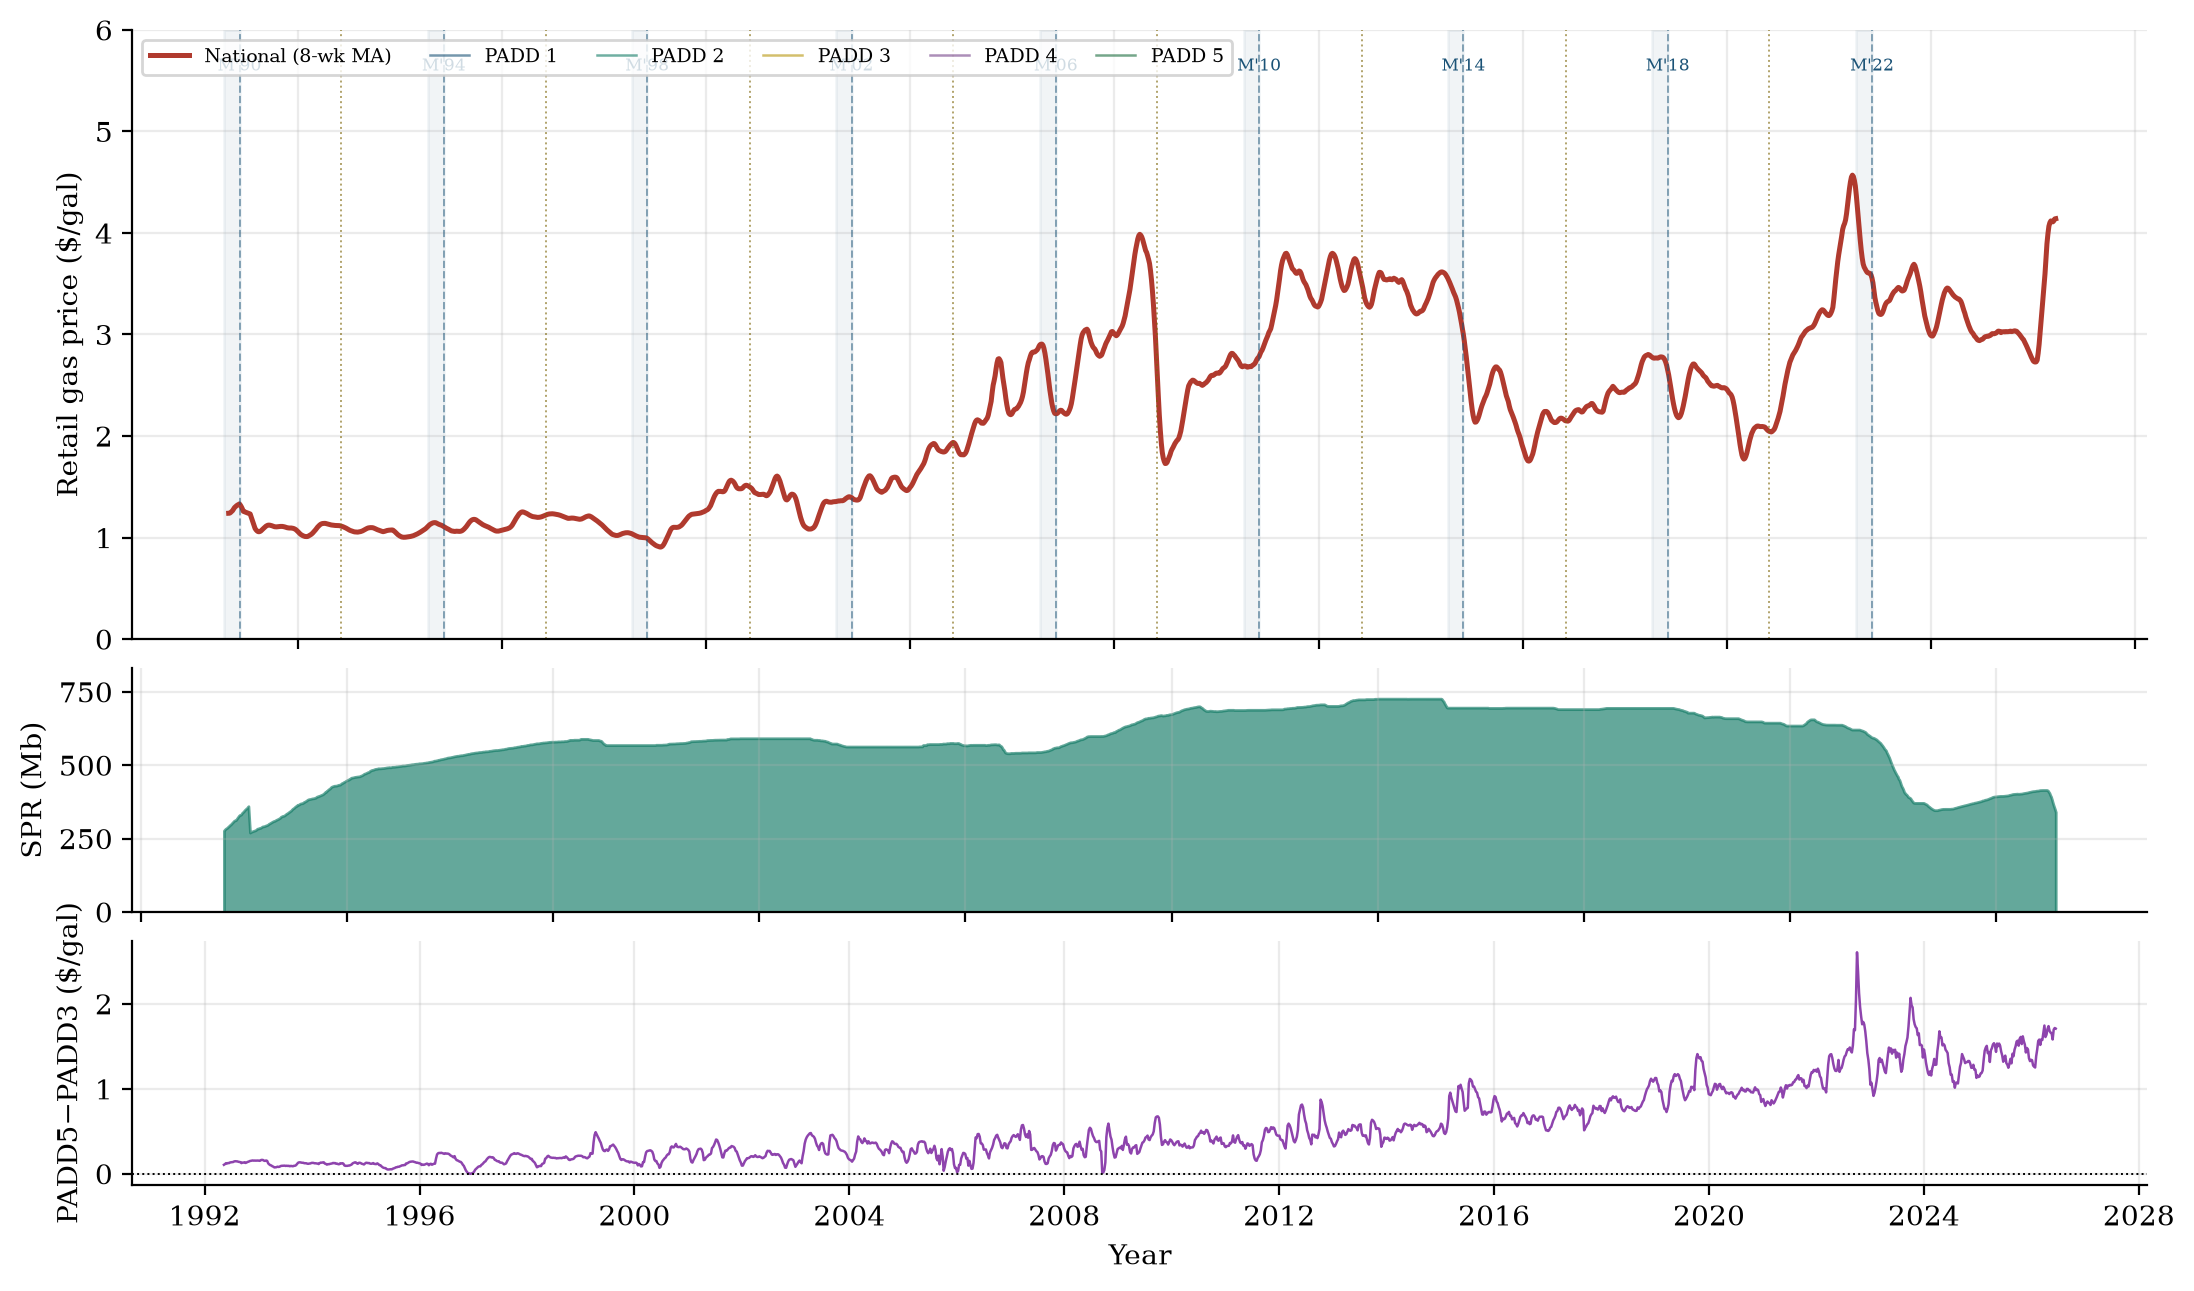
\includegraphics[width=\textwidth]{Figures/Figure1.png}
\caption{U.S.\ retail gasoline price and Strategic Petroleum Reserve stocks, 1974--2022. \textit{Upper panel}: weekly retail gasoline price (8-week moving average, \$/gallon); shaded bands mark the 16-week pre-midterm window for each cycle; dashed vertical lines indicate election day; key supply events are annotated. \textit{Lower panel}: SPR crude oil stocks (million barrels); the sharp decline from spring 2022 reflects the approximately 180\,Mb release during the run-up to the 2022 midterm. Sources: EIA GASREGW and WCSSTUS1 (calibrated series; see Section~\ref{sec:data}).}
\label{fig:timeline}
\end{figure}

\begin{figure}[!htbp]
\centering
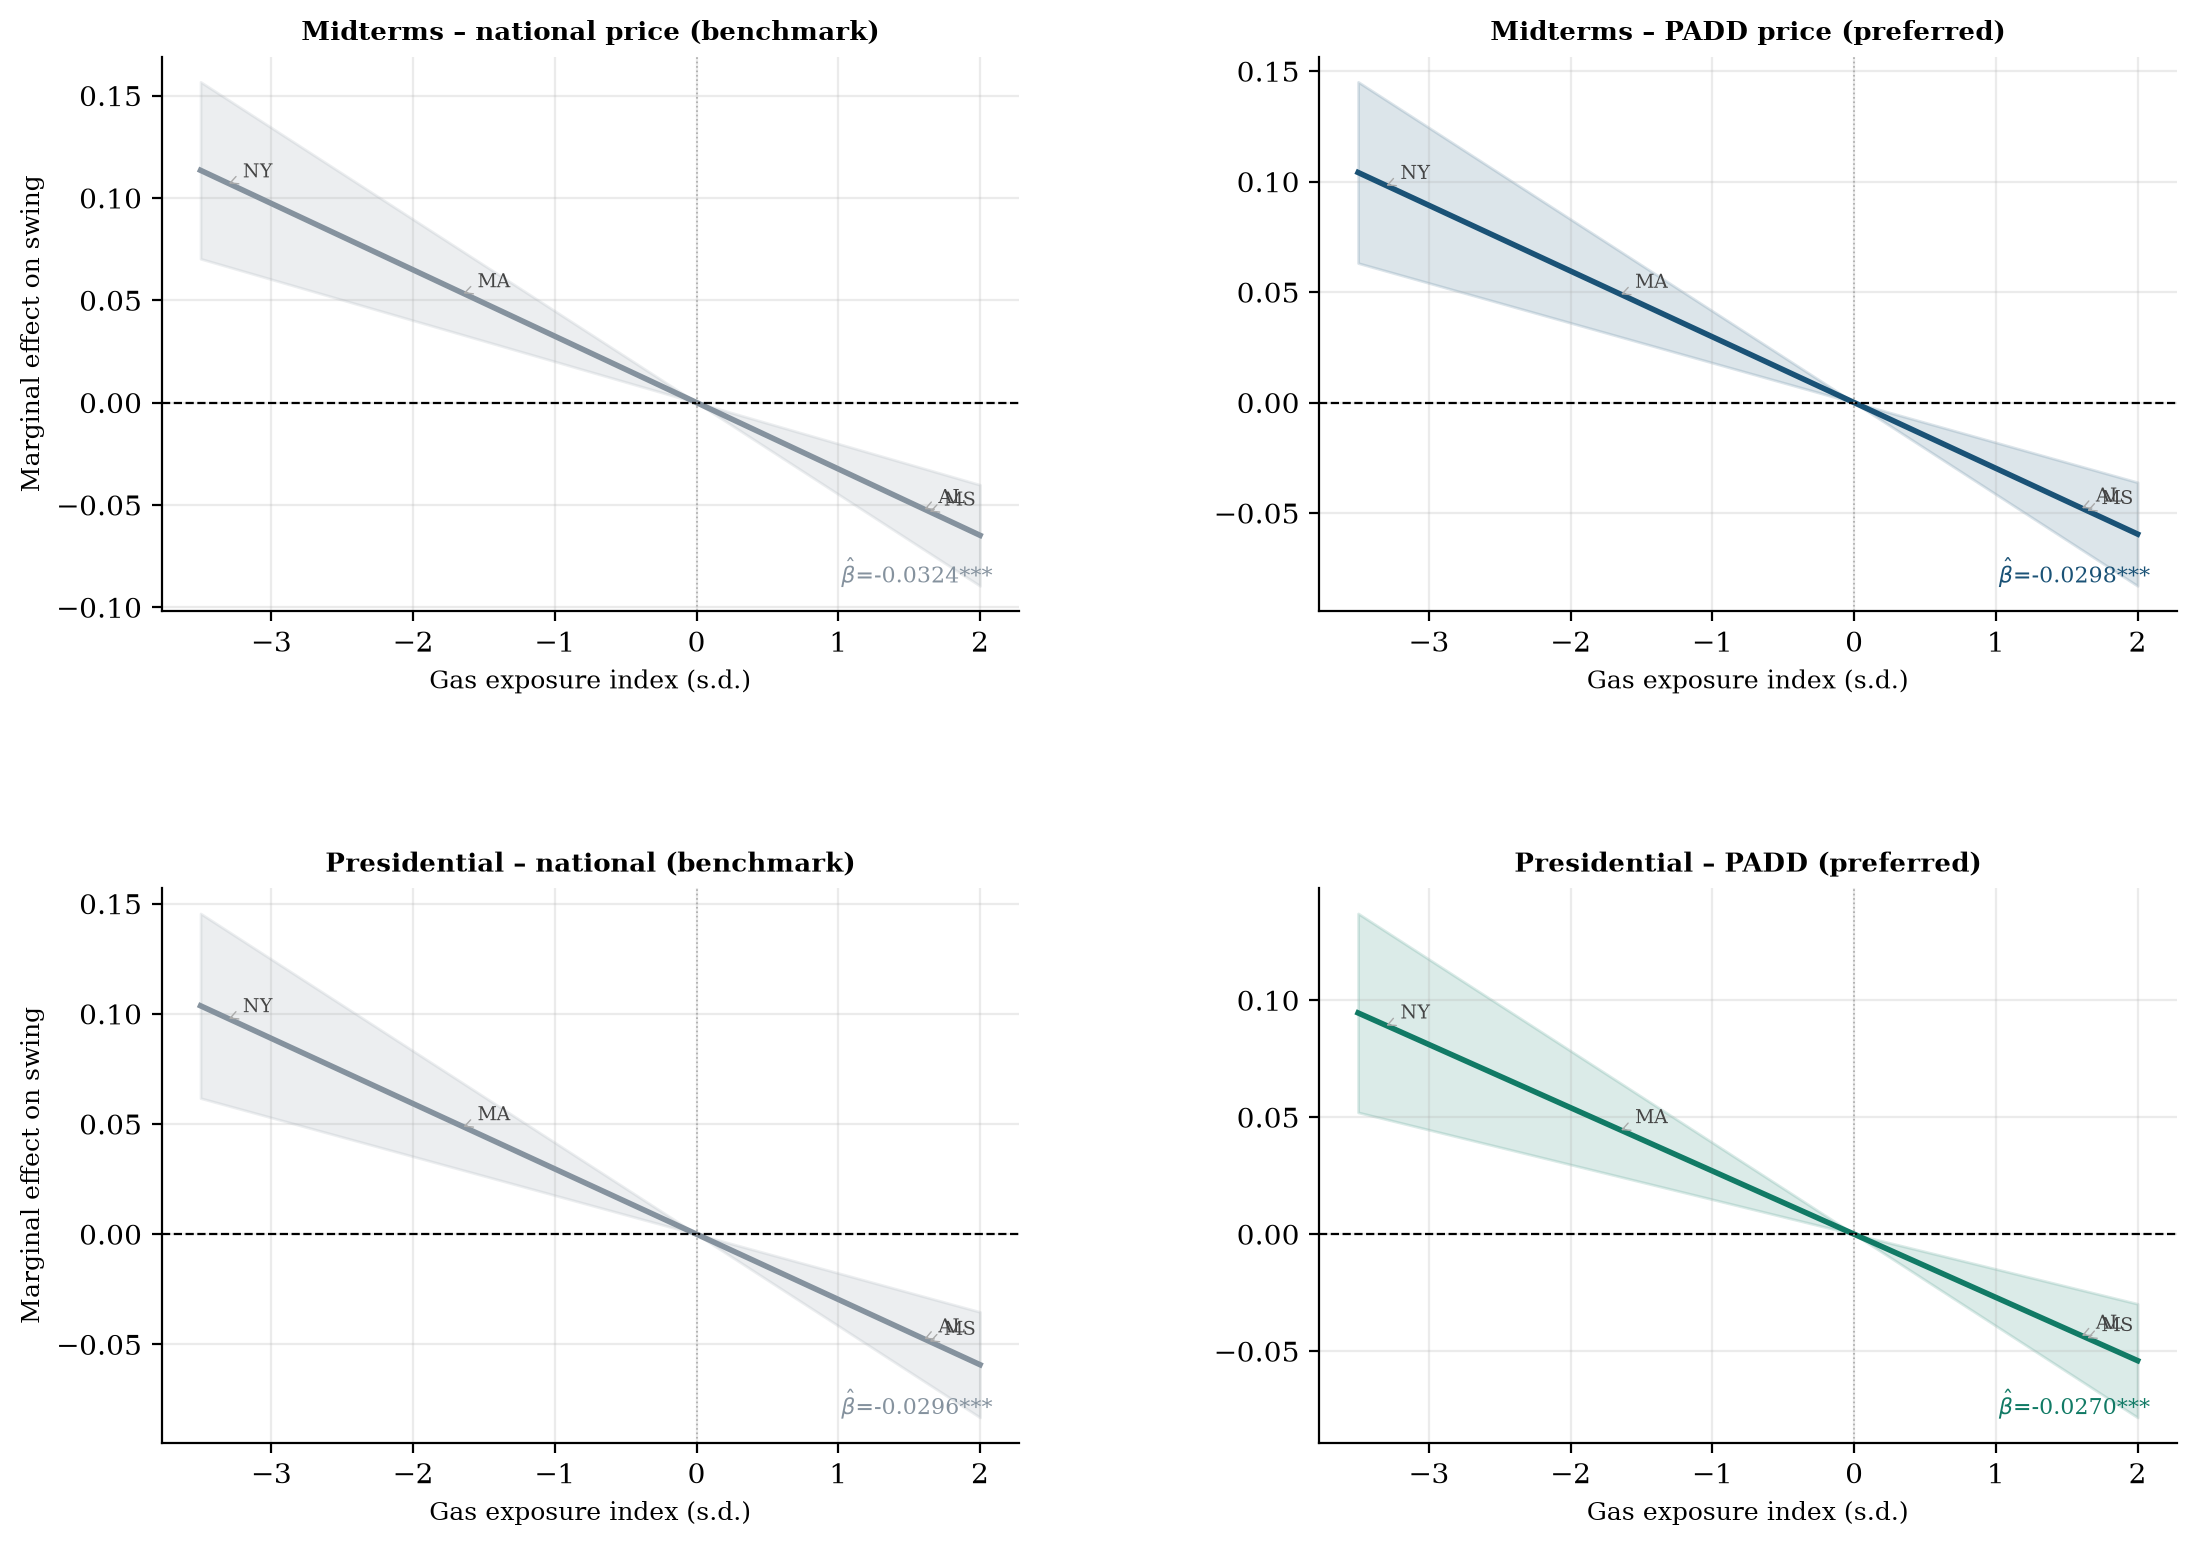
\includegraphics[width=\textwidth]{Figures/Figure2.png}
\caption{Marginal effect of gasoline prices on presidential party swing by state car dependence. Each panel shows $\partial(\Delta V_{s,t})/\partial\,\mathrm{Gas}_t = \hat\alpha + \hat\beta \cdot E_s$ as a function of $E_s$ (the gas exposure index, standardised to unit variance), for specifications M2 (year-over-year change), M5 (decay-weighted price $\mathrm{Gas}^W$, preferred), and M7 (six-month average). Shaded bands are 95\% confidence intervals; standard errors clustered by state. Selected state postal codes are annotated at their values of $E_s$. All estimates are from the primary sample (1994--2022, $N=239$); see Table~\ref{tab:main}.}
\label{fig:marginal}
\end{figure}

\begin{figure}[!htbp]
\centering
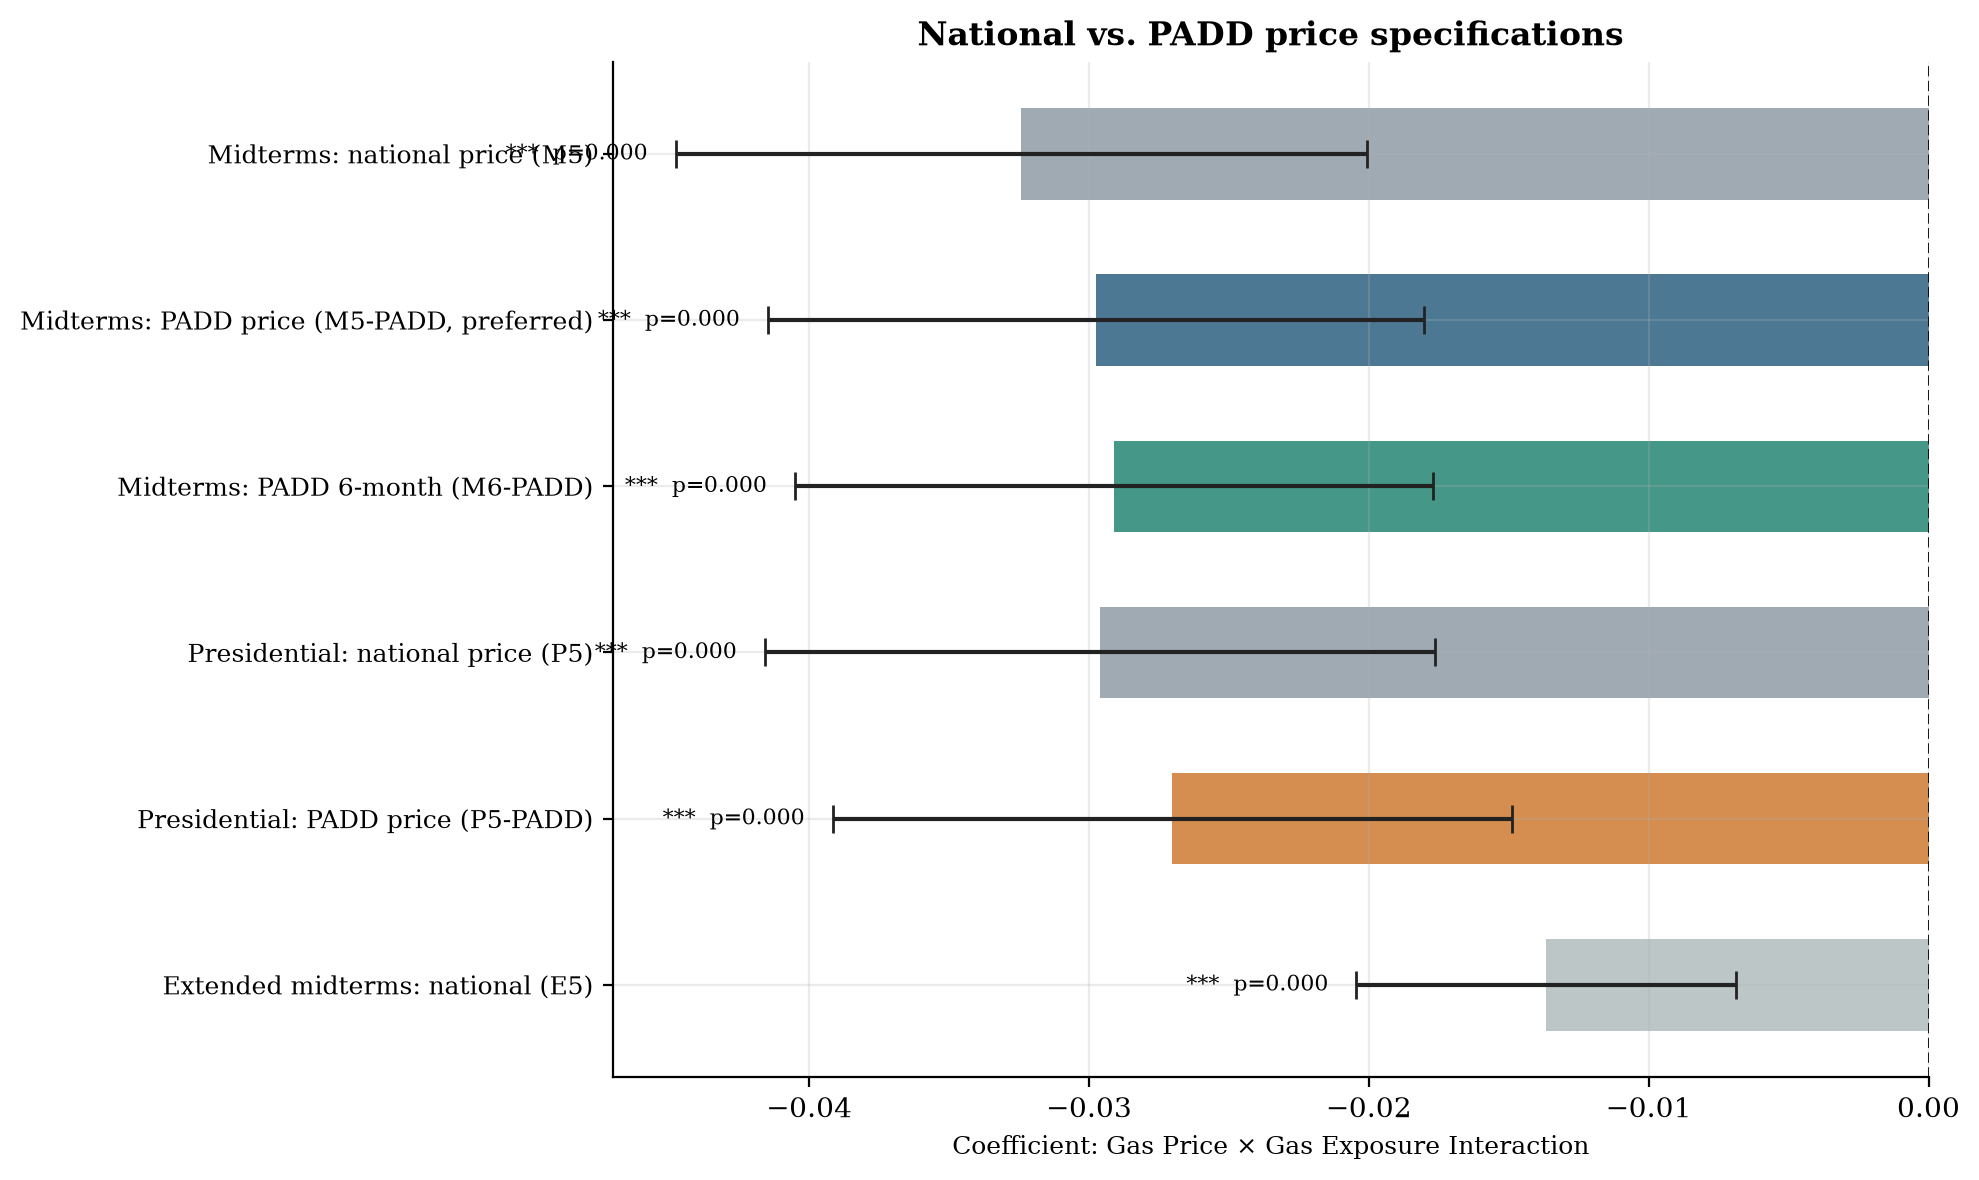
\includegraphics[width=0.88\textwidth]{Figures/Figure3.png}
\caption{Stability of the gas price $\times$ car dependence interaction across specifications. Point estimates and 95\% confidence intervals for the interaction coefficient $\hat\beta$ from specifications M2--M7, primary sample (1994--2022, $N=239$). All specifications include state and election-year fixed effects; standard errors clustered by state. Significance: $^{***}p<0.01$; $^{**}p<0.05$; $^{*}p<0.10$; n.s.\ not significant at conventional levels.}
\label{fig:forest}
\end{figure}

\begin{figure}[!htbp]
\centering
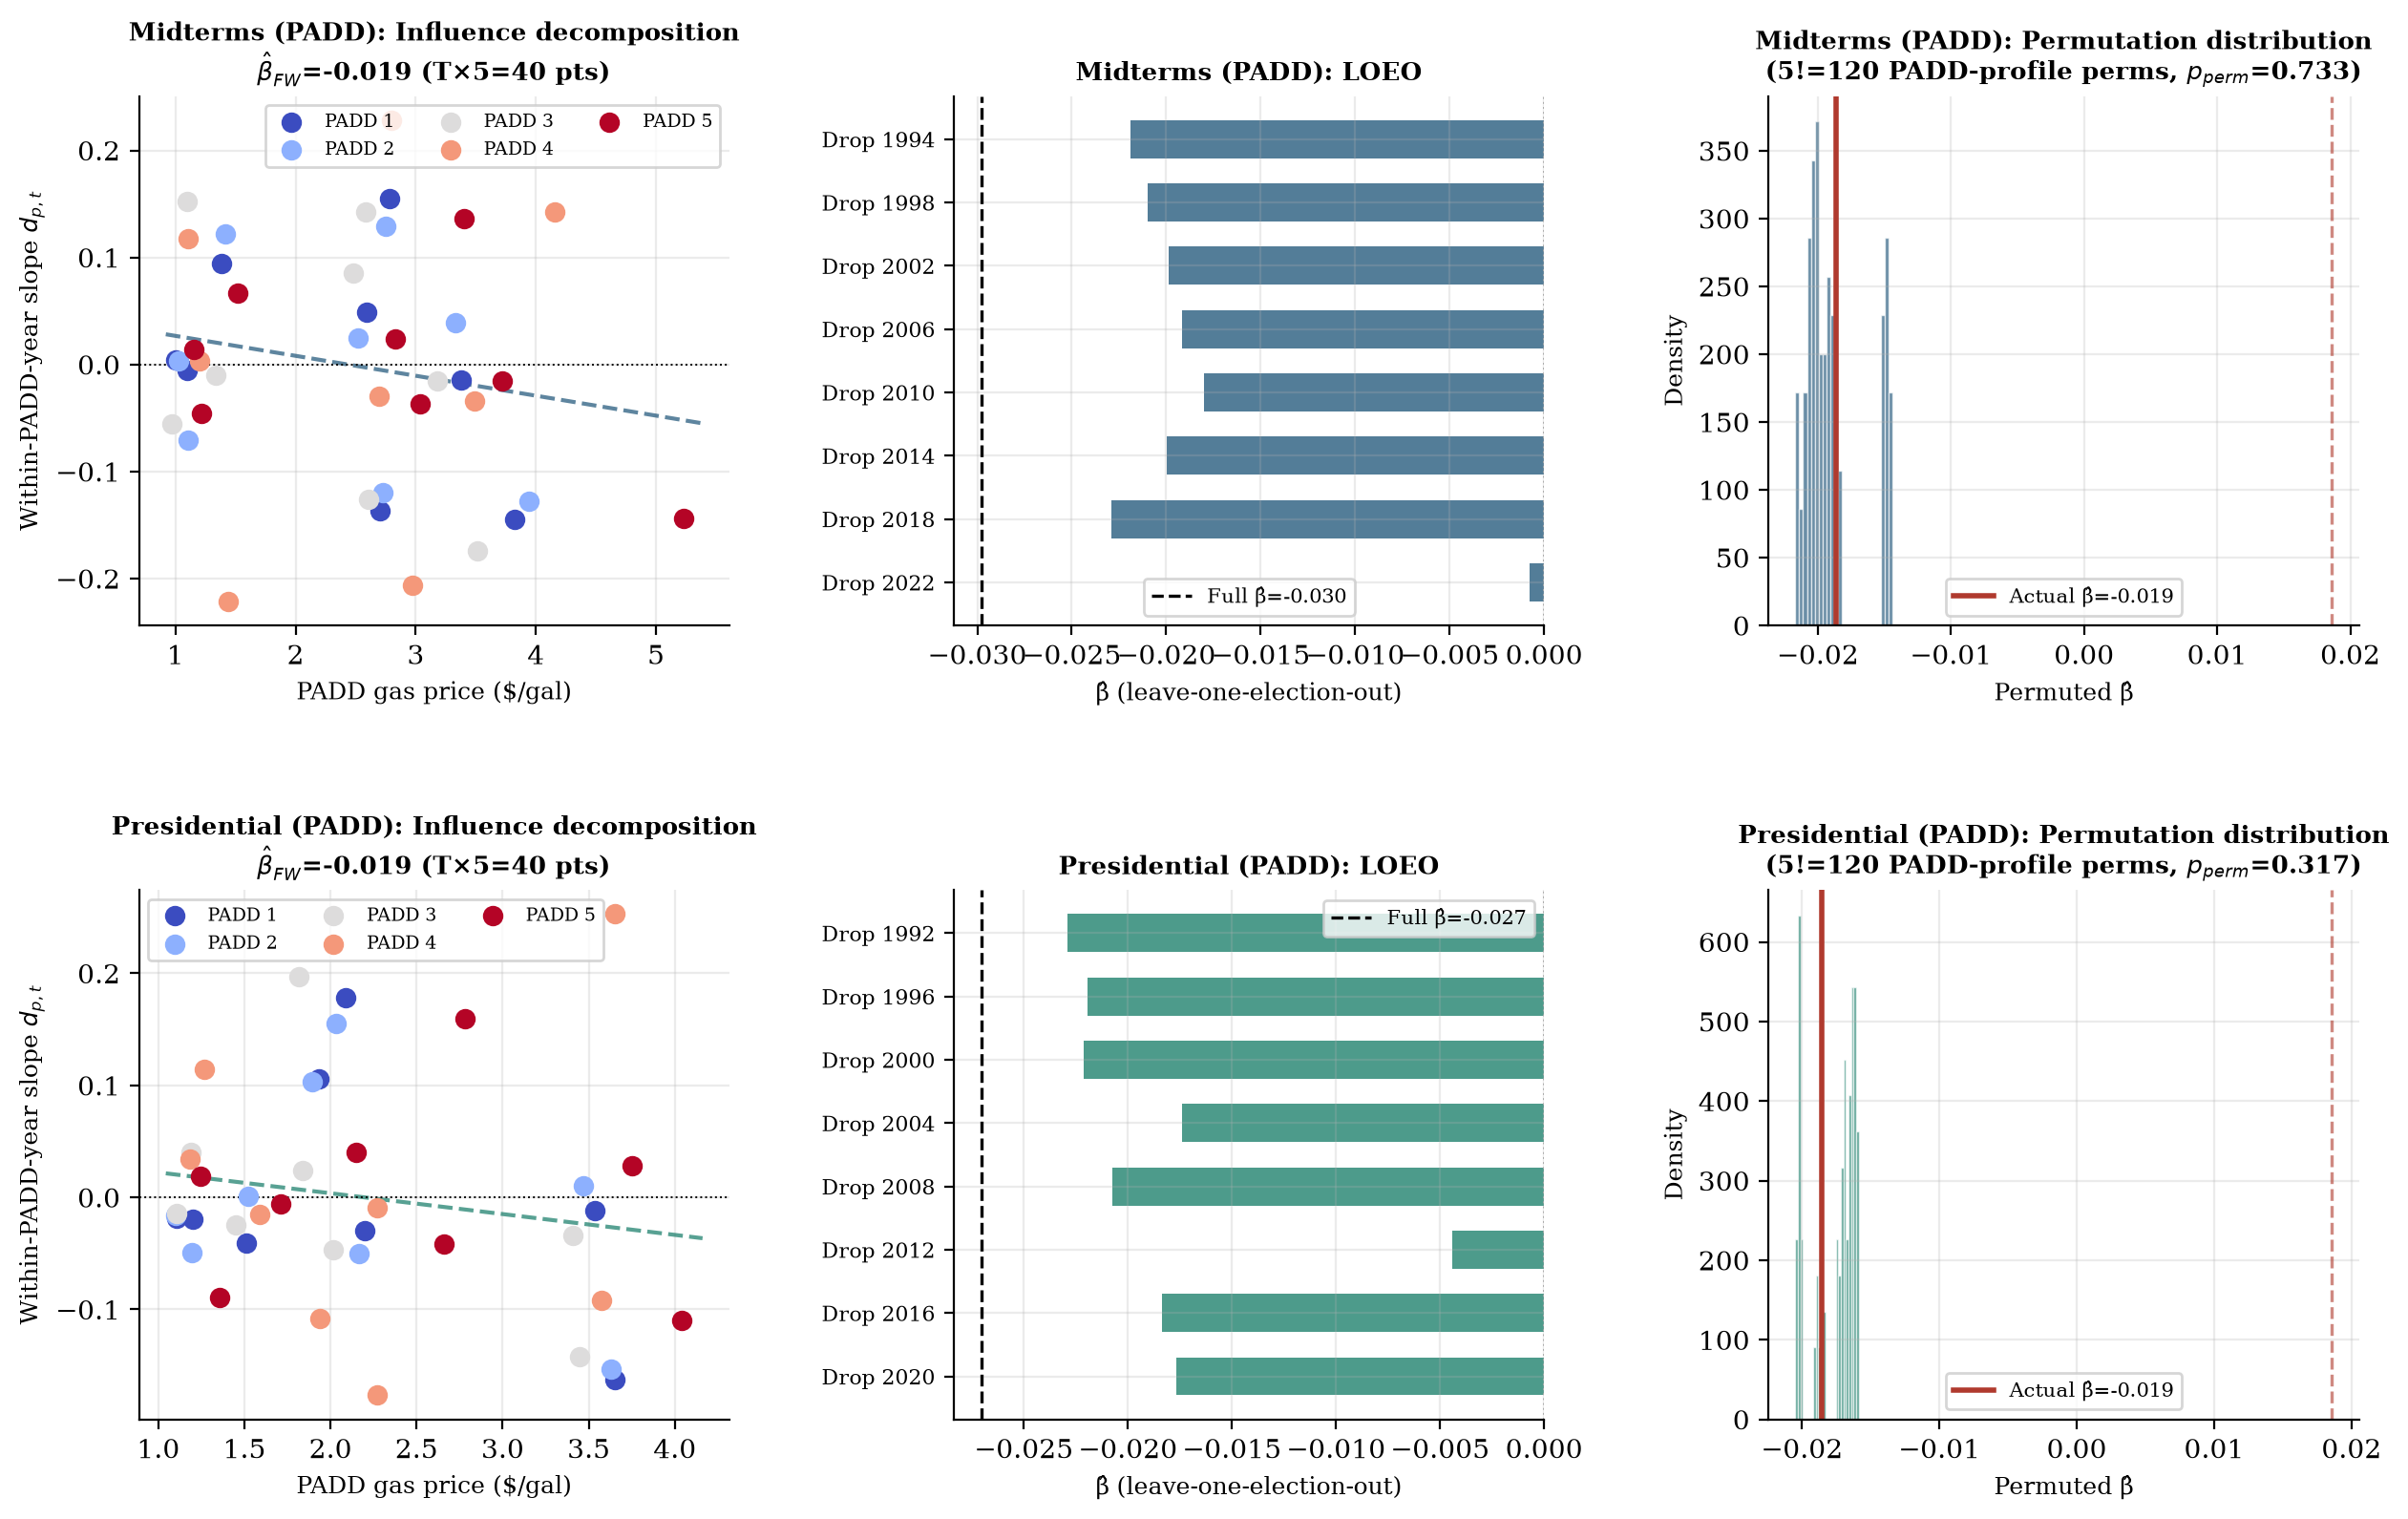
\includegraphics[width=\textwidth]{Figures/Figure4.png}
\caption{Election proximity, gasoline prices, and SPR deployment. \textit{Left panel}: raw mean weekly SPR drawdown (Mb) in four proximity regimes within the 16-week pre-midterm window, split by gas price regime (above and below historical median); positive values indicate net releases. \textit{Right panel}: mean retail gasoline price in the 16-week pre-election window for midterm cycles in which the incumbent ultimately gained seats versus lost seats; shaded bands are $\pm$1.96 standard errors of the mean. Both panels report unadjusted group means; the patterns are descriptive and should not be interpreted as regression-adjusted causal estimates (see Table~\ref{tab:timing} and Section~\ref{sec:results}).}
\label{fig:proximity}
\end{figure}

\end{document}